Once the experiment has been conducted and the data has been recorded, 
physicists might be interested in asking questions such as,
did one or did one not establish a discovery? Or,
how well does an alternate model describe this discovery?
The first question has to do with the goodness of the fit of the 
observed data to the good and old Standard Model,
while the second question has to do with hypotheses testing and the derivation of 
confidence intervals and upper limits~\cite{Stats-for-pedestrian}.
In order to answer these questions, one needs to first define the null hypothesis $H_0$ and
the alternative hypothesis $H_1$.
The definition of $H_1$ and $H_0$ depends of the specific physics problem, using the tone
of the particle physics, for search for a new signal process, the null hypothesis $H_0$ is 
assuming only the background is observed, the alternative hypothesis $H_1$ is assuming 
one observes both signal and background; for problems such as setting upper limits,
this definition is reversed.

It is common to refer to the \textit{p-value} to quantity the deviation from the null hypothesis, 
which is defined as:
\[
p = \int_{x_{obs}}^\infty g(x|H_0) dx,
\]
where $g(x|H_0)$ is the probability density function of observing a quantity
$x$ given the null hypothesis, and $x_{obs}$ is the observed value. The p-value derivation 
is shown illutratively in Figure~\ref{fig:stats:pvalue}, together with $\alpha$, 
which is defined as:
\[
\alpha = \int_{x_{5\sigma}}^\infty g(x|H_0) dx,  
\]
where $x_{5\sigma}$ is the observed value that corresponds $5\sigma$ deviation 
from the null hypothesis. 
One can therefore claim a discovery if the observed p-value $p < \alpha$ (equivalently, 
the background-only null hypothesis is rejected with a probability $1-p$).
Another commonly used statistic jargon is the \textit{confidence level} ($CL$),
which is defined as:
\[
CL   = \int_{ -\infty}^{x_{5\sigma}} g(x|H_0) dx \equiv 1- p .
\]
Lastly, the p-value is oftenly converted to a significance $Z$, 
defined as the number of standard deviations above the mean of a Gaussian distribution.
The relation between the p-value and $Z$ is given by:
\[
Z=\Phi^{-1} (1-p),
\]
where $\Phi_{-1}$ is the quantile function of the standard Gaussian distribution.
The discovery of signal, as mentioned before, needs to be rejecting the background-only hypothesis
with at least $Z \ge 5$, which corresponds to a p-value of $2.87 \times 10^{-7}$.
In the case of setting upper limits, for excluding the signal hypothesis, p-value is by convention 
required be less than 0.05 (95\% confidence level), which is equivalent to $Z = 1.64$.
This value is also used for setting upper limits in chapter~\ref{sec:search for dihiggs}.
N.B.\ In chapter~\ref{sec:search for dihiggs}, 
the $CL$ used for setting upper limits is calculated by the $CL_s$ method~\cite{CLs}
where $CL_s$ is (unfortunately named $CL_s$) given by:
\[
    CL_s   =  \frac{p_{s+b}}{1-p_b},
\]
where $p_{s+b}$ and $p_b$ are the confidence leveles for the signal-plus-background hypothesis
and the background-only hypothesis, respectively. 
The reason for using the $CL_s$ instead of the $p_{s+b}$ is that, in case of an experiment 
with low sensitivity, $1-p_b$ becomes small, and hence the signal will not 
be excluded even with a small p-value. 

\begin{figure}[htbp]
    \centering
    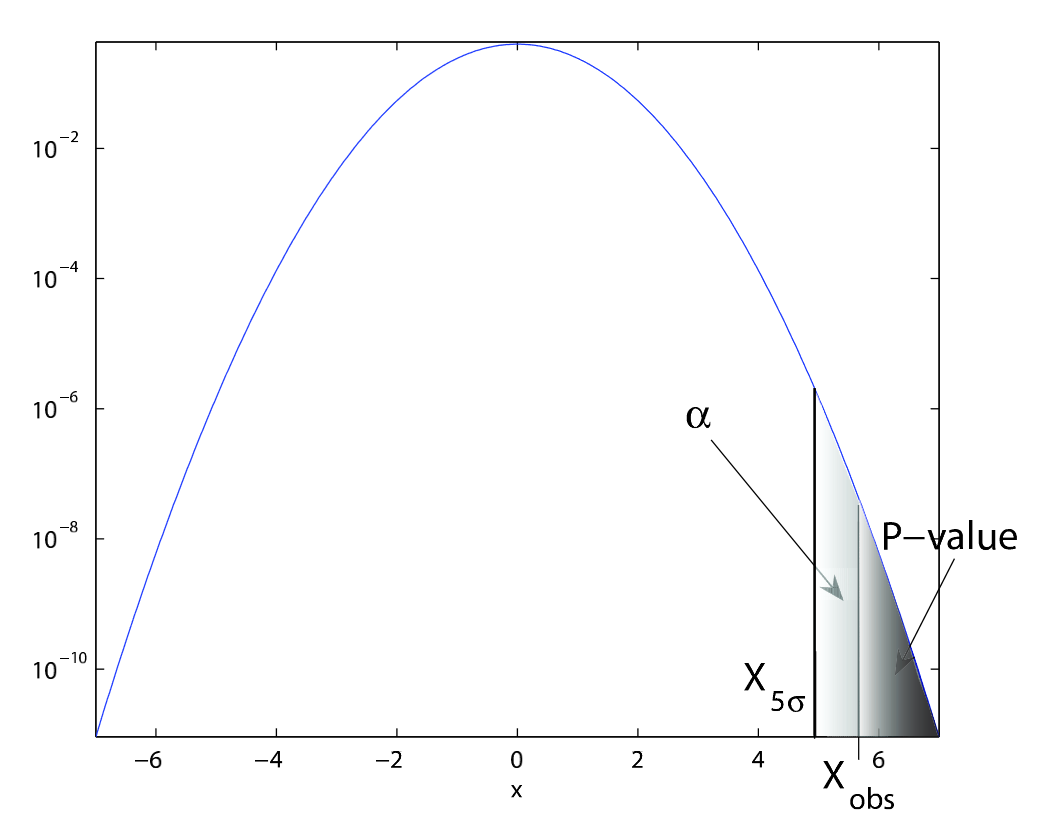
\includegraphics[width=0.6\textwidth]{theory/plots/pvalue.png}
    \caption{An illustration showing the control area $\alpha$ and the p-value of a Gaussian distribution. Note, in this 
    example $X_{obs} > X_{5\sigma}$. Image taken from Ref.\cite{Stats-for-pedestrian}}.
    \label{fig:stats:pvalue}
\end{figure}









\subsection{Test statistics}
In terms of hypothesis testing, 
A test statistic is a quantity calculated from data,
which can be used to estimate how probable is the result 
that we observe with respect to some null hypothesis.
Due to the Neyman-Pearson lemma~\cite{Neyman-Pearson}, the most powerful test statistic
one can construct is given by:
\[
Q  = \frac{L(H_1)}{L(H_0)},
\]
where $L(H_1)$ and $L(H_0)$ are the likelihood of the hypothesis $H_1$ and $H_0$, respectively.
The likelihood function is defined 

\subsection{Look elsewhere effect}
We can specify an hypothesis with a specific Higgs mass but had we observed some possible signal
we should take into account that this signal could be a fluctuation which could be observed anywhere in
our sensitivity range [2]. Here we change the signal hypothesis from a Higgs with a specific mass mH to
a Higgs with some mass in the observed region. It is not clear how to take these effects into account. One
common way is to degrade the observed p-value by multiplying it by the size of the sensitivity region
divided by the experimental resolution. A common claim is that the control region for discovery is so
small that "who cares".... Another common belief is that the "look elsewhere effect" is the reason for the
habit of defining a discovery as a 5$\sigma$ and not for example 4$\sigma$, because even if you quote 5$\sigma$ your effective
significance is lower.

The look-elsewhere effect is accounted by calculating the global significance
following Ref.\cite{global-significance}, using the up-crossing method:
\[ p_\text{global} = p_\text{local} +  N_\text{up} e^{-1/2(Z^2_\text{local} - Z^2_\text{ref})},
\]
where the $p_\text{local}$ and $p_\text{global}$ are the local and global p-values, and
$Z_\text{ref}$ is chosen for p=0.5 (corresponding to 0~$\sigma$ significance level), 
and $N_\text{up}$ is the number of times the local p-value curve crossing the reference line (in this case,
p=0.5) in the upwawrd direction.
The estimated global significance is $2.1^{+0.4}_{-0.2} \sigma$.
